\section{Extensive Form}
Extensive form is used to describe a multi-stage game.
\begin{definition}
    An \uimpt{extensive form} specifies a game tree, player functions, information sets, and payoffs.
\end{definition}
The game tree is a set of nodes connected by directed branches where there exists a root node such that each node (final or non-final) has at most 1 incoming branch, and can be reached uniquely from the root. We denote the non-final nodes to be $h$. \\
The players is represented by a set $N := \{1, 2, \dots, n\}$, where each player has functions $P(h)$, and payoffs $u_i(h_f)$ (final nodes). \\
An information set is what cannot be distinguished by a player (a set of nodes). Within the same information set, it must be the same player to move, the same moves available. Every non-final node is in an information set, which can be singleton, and they form an information partition. \\
There are two types of multi-stage games. The game is either \impt{perfect information} (players know all previous information, and information sets are all singletons) or \impt{imperfect information} (at least one non-singleton information) set. \\
The strategy of a player represents what one should do in every information set (a complete contingent plan) even if some information sets are ``unreachable''.
\begin{definition}
    Let $I_i$ be an information set for player $i$. For all $I_i$, $A(I_i)$ is the set of actions available at $I_i$. A strategy profile is $(s_1, \dots, s_n)$ where for all $I_i$, $s_i(I_i)$ is an action taken by $i$ at $I_i$ and we have $s_i(I_i) \in A(I_i)$.
\end{definition}
We solve the game that ensures credible threats or behaviours (there can be other Nash equilibria) by looking for ``smaller games'' and determine what players would do in that situation.
\begin{definition}
    A \uimpt{subgame} is a subset of nodes such that it contains a specific $h \in H$ and contains all $\text{SUCC}(h)$. If $h \in I_i$ is in a subgame and $h' \in I_i$, then $h'$ is also in the same subgame.
\end{definition}
\begin{definition}
    A \uimpt{subgame perfect equilibrium} is a strategy profile that induces a Nash equilibrium in every subgame.
\end{definition}
We find this kind of equilibrium through \impt{backward induction}. \\
In finite perfect information games, all subgame perfect equilibria can be obtained by backward induction.

\subsection{Perfect Information Games}
\begin{definition}
    \uimpt{Competitive games} are a special class of zero-sum games, where outcomes are only victory, tie, or loss, with $2$ players and finite moves.
\end{definition}
\begin{theorem}
    \uimpt{Zermelo's theorem} states that in a competitive game, either player $A$ has a strategy that guarantees ``victory'', or player $B$ has a strategy that guarantees ``victory'', or both players have a strategy that guarantees ``tie''.
\end{theorem}
This is shown through induction.

\subsection{Bargaining}
We consider a group of agents who need to divide a resource among themselves. A Rubinstein-Stahl models this by players making offers, which can be turned down. \\
A simple model is a single round of negotiation (\impt{ultimatum game}) which consists of $2$ players. Player $1$ makes offer $x_1$ for itself, where $x_1 \in [0, 1]$ and player $2$ decides Y or N. If player $2$ choose Y, they get $(x_1, 1 - x_1)$; if player $2$ choose N, they get $(0, 0)$. \\
In this case, the subgame perfect Nash equilibrium includes $r_2(x_1)=Y$, as it is always the best response of player $2$ ($1 - x_1 \ge 0$). Since player $1$ can choose any $x_1$, it will choose $x_1$ that maximizes its profit. Thus, the SPE is $r_1(\cdot) = 1$, and $r_2(x_1) = Y$. Another best response by player $2$ is to only say yes when player $1$ offers something strictly less than $1$, but in this case, there is no optimal strategy for player $1$, so it is not part of the SPE. \\
Then, we consider a $2$-round model, where player $2$ has a chance to make an offer $x_2 \in [0, 1]$ if the first round of bargaining did not work. However, delay is costly. Thus, if agreement is reached in second round, the payoffs will be $(\delta(1 - x_2), \delta x_2)$, where $\delta \in (0, 1)$. The extensive form is:
\begin{center}
    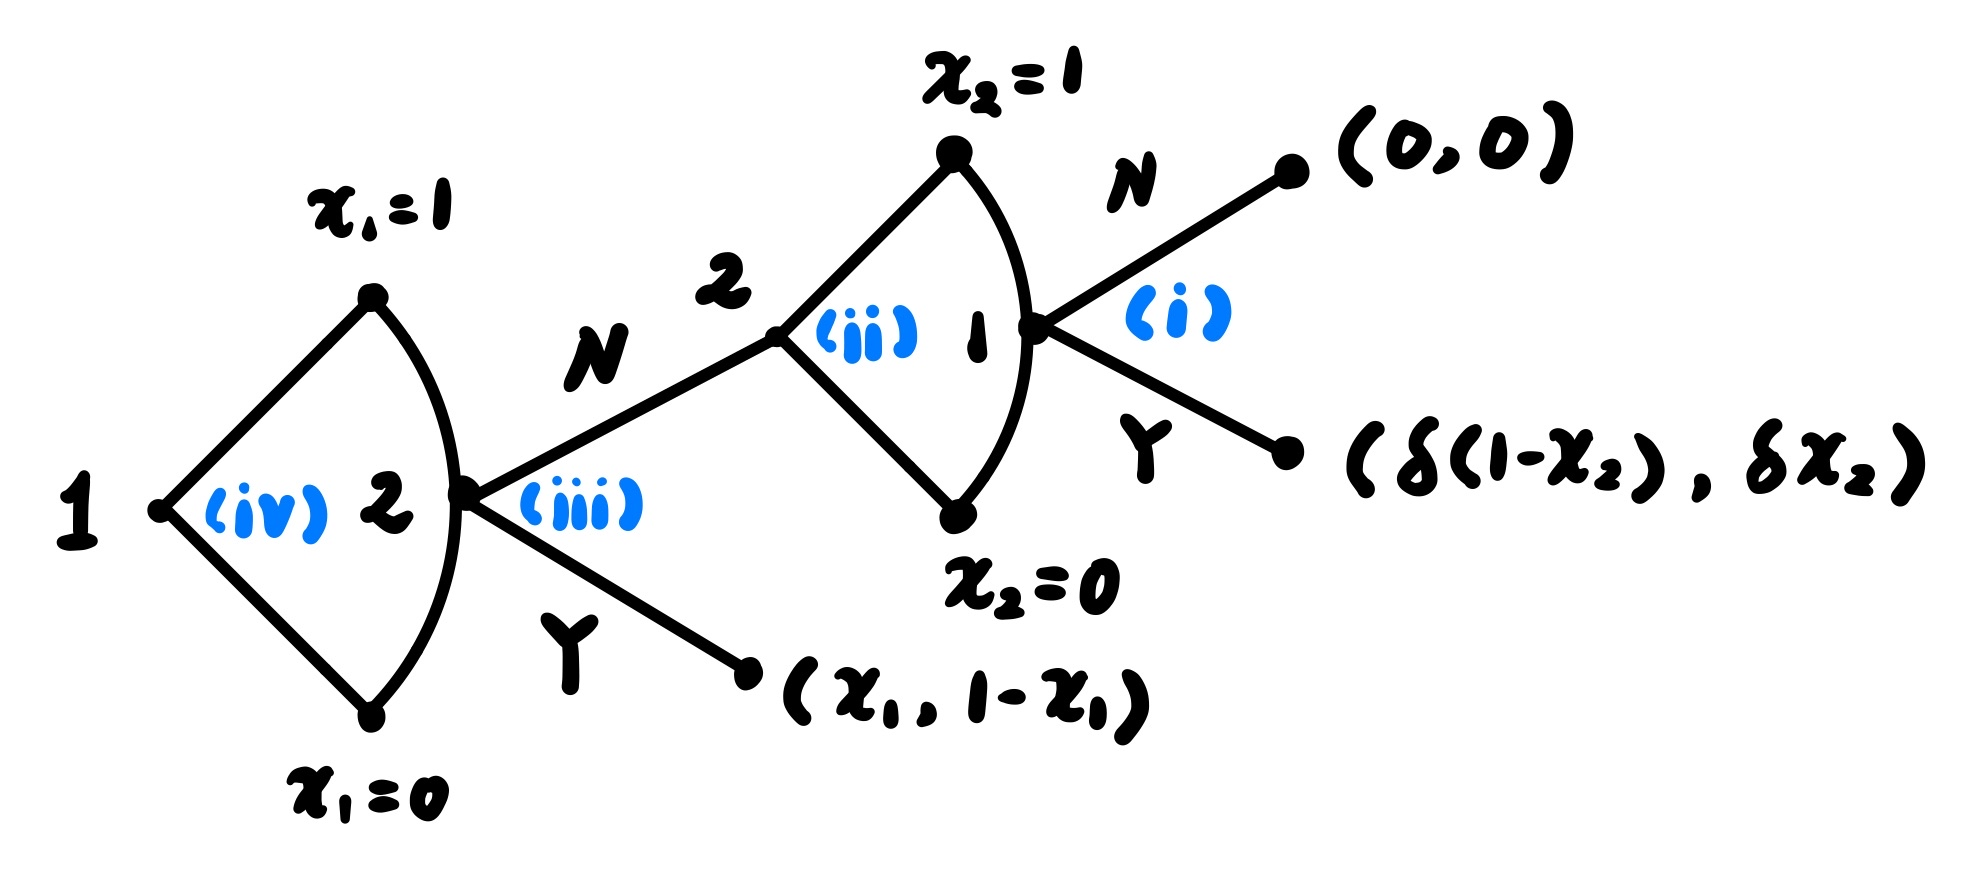
\includegraphics[scale = 0.2]{3/2_round.png}
\end{center}
The game at (ii) is an ultimatum game, which gives a payoff of $(0, \delta)$, where player $2$ choose to offer $x_2 = 1$ and player $1$ responds with Y. \\
We move one step back, we want to compare $1 - x_1$ and $\delta$. Thus, at (iii), the best response of player $2$ is:
$$r_2^*(x_1) = \begin{cases}
    Y & 1 - x_1 \ge \delta \to x_1 \le 1 - \delta \\
    N & 1 - x_1 < \delta \to x_1 > 1 - \delta
\end{cases}$$
This implies the best response at (iv) by player $1$ is $x_1 = 1 - \delta$, as it is the highest acceptable offer. \\
The SPE is then described to be: $r_1^*(\cdot) = 1 - \delta, r_2^*(x_1), r_2^*(x_1, N) = 1, r_1^*(x_1, N, x_2) = Y$. \\
Finally, we consider a ``not-so-simple'' model about this game. In real applications, players do not know the number of rounds or offers, there is uncertainty about time. This model uses an \impt{infinite horizon} model, that is if an offer is rejected, another one is made next period, but delay is costly such that if the negotiation is too long, nothing is left. The discount rate for each player is $\delta_1$ and $\delta_2$. The more impatient the player is, the smaller their $\delta$ would be. Note that in this case, a subgame at start of round $n$ is identical to the subgame at start of round $n + 2$. Thus, for simplicity, we focus on stationary strategies, where players act similarly in similar situations, regardless of calendar date. \\
For player $i$, when offering, offers to keep $x_i^*$; when accepting, will accept anything above the threshold of $\underbar{x}_i$. Suppose no offers are accepted when $1 - x_1^* < \underbar{x}_2$ and $1 - x_2^* < \underbar{x}_1$. For the game to end somewhere, at least one of the inequality is violated. \\
In this case, in a certain round, assume player $1$ is making an offer, and player $2$ decides to accept the offer. This means $1 - x_1^* \ge \underbar{x}_2$. To maximize profit, $x_1^* = 1 - \underbar{x}_2$. \\
Then, we trace back one step, where player $2$ is making an offer in the previous round, offering $x_2$. If player $1$ accepts, it gets $1 - x_2$; if it declines, it gets $\delta_1 x_1^*$ (from next round). This means player $1$ will accept as long as $1 - x_2 \ge \delta_1 x_1^*$. \\
Now, we think about player $2$ making this offer. If it offers such that $1 - x_2 \ge \underbar{x}_1$, player $2$ gets at most $x_2 = 1 - \underbar{x}_1$; if it offers such that $1 - x_2 < \underbar{x}_1$, player $1$ will reject, and in the next round, player $2$ will get $\delta_2 (1 - x_1^*)$. However, it is easily shown that $1 - \underbar{x}_1 \ge \delta_2 (1 - x_1^*)$. This means $x_2^* = 1 - \underbar{x}_1$. \\
By tracing one more step back, similar to the second step in analysis, we have $\underbar{x}_2 = \delta_2 x_2^*$. \\
This gives us a system of equations:
$$\begin{cases}
    x_i^* = 1 - \underbar{x}_j \\
    \underbar{x}_i = \delta_i x_i^*
\end{cases}$$
for $i, j \in \{1, 2\}$. This solves to:
$$\begin{cases}
    x_i^* = \frac{1 - \delta_j}{1 - \delta_i\delta_j} \\
    \underbar{x}_i = \delta_i \cdot \frac{1 - \delta_j}{1 - \delta_i\delta_j}
\end{cases}$$
If player $1$ initiates this bargaining, the payoff is thus $(x_1^*, 1 - x_1^*)$ described above. By setting $\delta_i \approx 1$ and $\delta_i = 0$, we can obtain four situations of payoffs. \\
The role of patience is that say each stage lasts $\Delta > 0$, and players use interest rate $r_i > 0$ to indicate patience where $\delta_i = e^{-r_i \Delta}$. Fast offering, which is $\Delta \to 0$, will yield that:
$$x_1^* \to \frac{r_2}{r_1 + r_2}, \underbar{x}_1 \to \frac{r_2}{r_1 + r_2}$$


\newpage